\subsection{Störungsunterdrückung - LQRI}
Um Störung und Modelfehler zu unterdrücken greift man zum LQRI, welcher zusätzlich zum standard LQR-Regler noch ein integratives Verhalten eingeführt wird. Um Störungen zu unterdrücken wird das Integral des Fehlers als neuer Zustand definiert: \[ v(t) = \int^t_0 e(\tau)d\tau = \int^t_0 (0-<(\tau))d\tau.\]
der neue Gesamtzustand lautet somit: \[\Tilde{x}(t) =\begin{bmatrix}
x(t) \\ v(t)
\end{bmatrix}\in \mathbb{R}^{n+m}\]

Die Ableitung des Zustands lautet
\begin{align*}
    \frac{d}{dt}\Tilde{x}(t) = \begin{bmatrix}A\cdot x(t) + B \cdot ( u(t) + w(t))\\-y(t)\end{bmatrix}\\
    = \underbrace{\begin{bmatrix}A&0\\-C & 0\end{bmatrix}}_{\Tilde{A}}\cdot\begin{bmatrix}x(t) \\v(t)\end{bmatrix}+\underbrace{\begin{bmatrix}B \\ 0 \end{bmatrix}}_{\Tilde{B}} \cdot(u(t)+w(t))
\end{align*}
Das neue System erfüllt im Gleichgewicht $\dot v = y(t) = 0$

\begin{figure}[H]
    \centering
    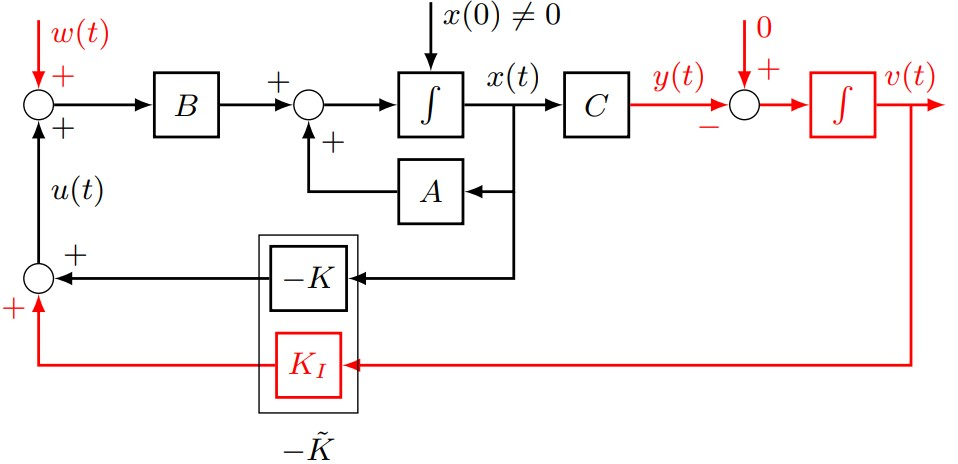
\includegraphics[width=0.8\linewidth]{images/08/LQRI.jpg}
    \caption{Standarddarstellung des LQRI}
\end{figure}

Die Standard LQR Formulierung kann nun mit den Matrizen $\Tilde{A}$ und $\Tilde{B}$ gelöst werden, wobei die Dimension der $Q$ Matrix angepasst werden muss:
\[\Tilde{Q} =\begin{bmatrix} Q & 0 \\ 0 & Q_I\end{bmatrix},\ Q_I = \begin{bmatrix}
    \gamma_1 & 0 & \dots & 0 \\
    0 & \gamma_2 & \dots & 0\\
    \vdots & \vdots &\ddots &   \vdots\\
    0 & 0 & \dots &\gamma_m
\end{bmatrix}\]
Mit $Q_I$ kann man einstellen, wie stark die Integratoren wirken sollen. Die Lösung des LQRI-Problems lautet:
\begin{align*}
    \{\Tilde{A},\Tilde{B},\Tilde{Q},R\}\rightarrow \Tilde{K}=[\,K, - K_I]\, \in \mathbb{R}^{m\times(n+m)},\\
    u(t) = -\Tilde{K}\cdot\Tilde{x}(t) = u_K + u_{K_I} = -K\cdot x(t) + K_I\cdot v(t).
\end{align*}
note: \begin{itemize}
    \item Die Matrix $\Tilde{K}$ ist statisch, sie muss für gegebene $\{\Tilde{A},\Tilde{B},\Tilde{Q},R\}$ nur einmal berechnet werden.
    \item Mit $Q = C^T \cdot C$ kann wiederum direkt $y(t)$ in der Kostenfunktion berücksichtigt werden. 
\end{itemize}